\documentclass{beamer}

\usefonttheme{professionalfonts} % using non standard fonts for beamer
\usefonttheme{serif} % default family is serif

\usepackage{hyperref}
%\usepackage{minted}
\usepackage{animate}
\usepackage{graphicx}
\def\Put(#1,#2)#3{\leavevmode\makebox(0,0){\put(#1,#2){#3}}}
\usepackage{color}
\usepackage{tikz}
\usepackage{amssymb}
\usepackage{enumerate}


\newcommand\blfootnote[1]{%

  \begingroup

  \renewcommand\thefootnote{}\footnote{#1}%

  \addtocounter{footnote}{-1}%

  \endgroup

}

\makeatletter

%%%%%%%%%%%%%%%%%%%%%%%%%%%%%% Textclass specific LaTeX commands.

 % this default might be overridden by plain title style

 \newcommand\makebeamertitle{\frame{\maketitle}}%

 % (ERT) argument for the TOC

 \AtBeginDocument{%

   \let\origtableofcontents=\tableofcontents

   \def\tableofcontents{\@ifnextchar[{\origtableofcontents}{\gobbletableofcontents}}

   \def\gobbletableofcontents#1{\origtableofcontents}

 }

%%%%%%%%%%%%%%%%%%%%%%%%%%%%%% User specified LaTeX commands.

\usetheme{Malmoe}

% or ...

\useoutertheme{infolines}

\addtobeamertemplate{headline}{}{\vskip2pt}

\setbeamercovered{transparent}

% or whatever (possibly just delete it)

\makeatother

\begin{document}
\title[PFLOCK report]{PFLOCK Report}
\author[AC]{Andres Calderon}
\institute[Summer'19]{University of California, Riverside}
\makebeamertitle
\newif\iflattersubsect

\AtBeginSection[] {
    \begin{frame}<beamer>
    \frametitle{Outline} 
    \tableofcontents[currentsection]  
    \end{frame}
    \lattersubsectfalse
}

\AtBeginSubsection[] {
    \begin{frame}<beamer>
    \frametitle{Outline} 
    \tableofcontents[currentsubsection]  
    \end{frame}
}

\section{Extended test on MF Algorithm}

\begin{frame}{Extended tests on MF Algorithm}
    \begin{itemize}
        \item Some confusing results in LA\_50K and LA\_100K (maybe due to skew data).
        \item Using uniform dataset to find some pattern.
        \item Quadtree not always generate the same number of partitions even if the same \texttt{MaxEntries} is used.
    \end{itemize}
\end{frame}

\begin{frame}{Extended tests on MF Algorithm (LA\_50K dataset)}
    \centering
    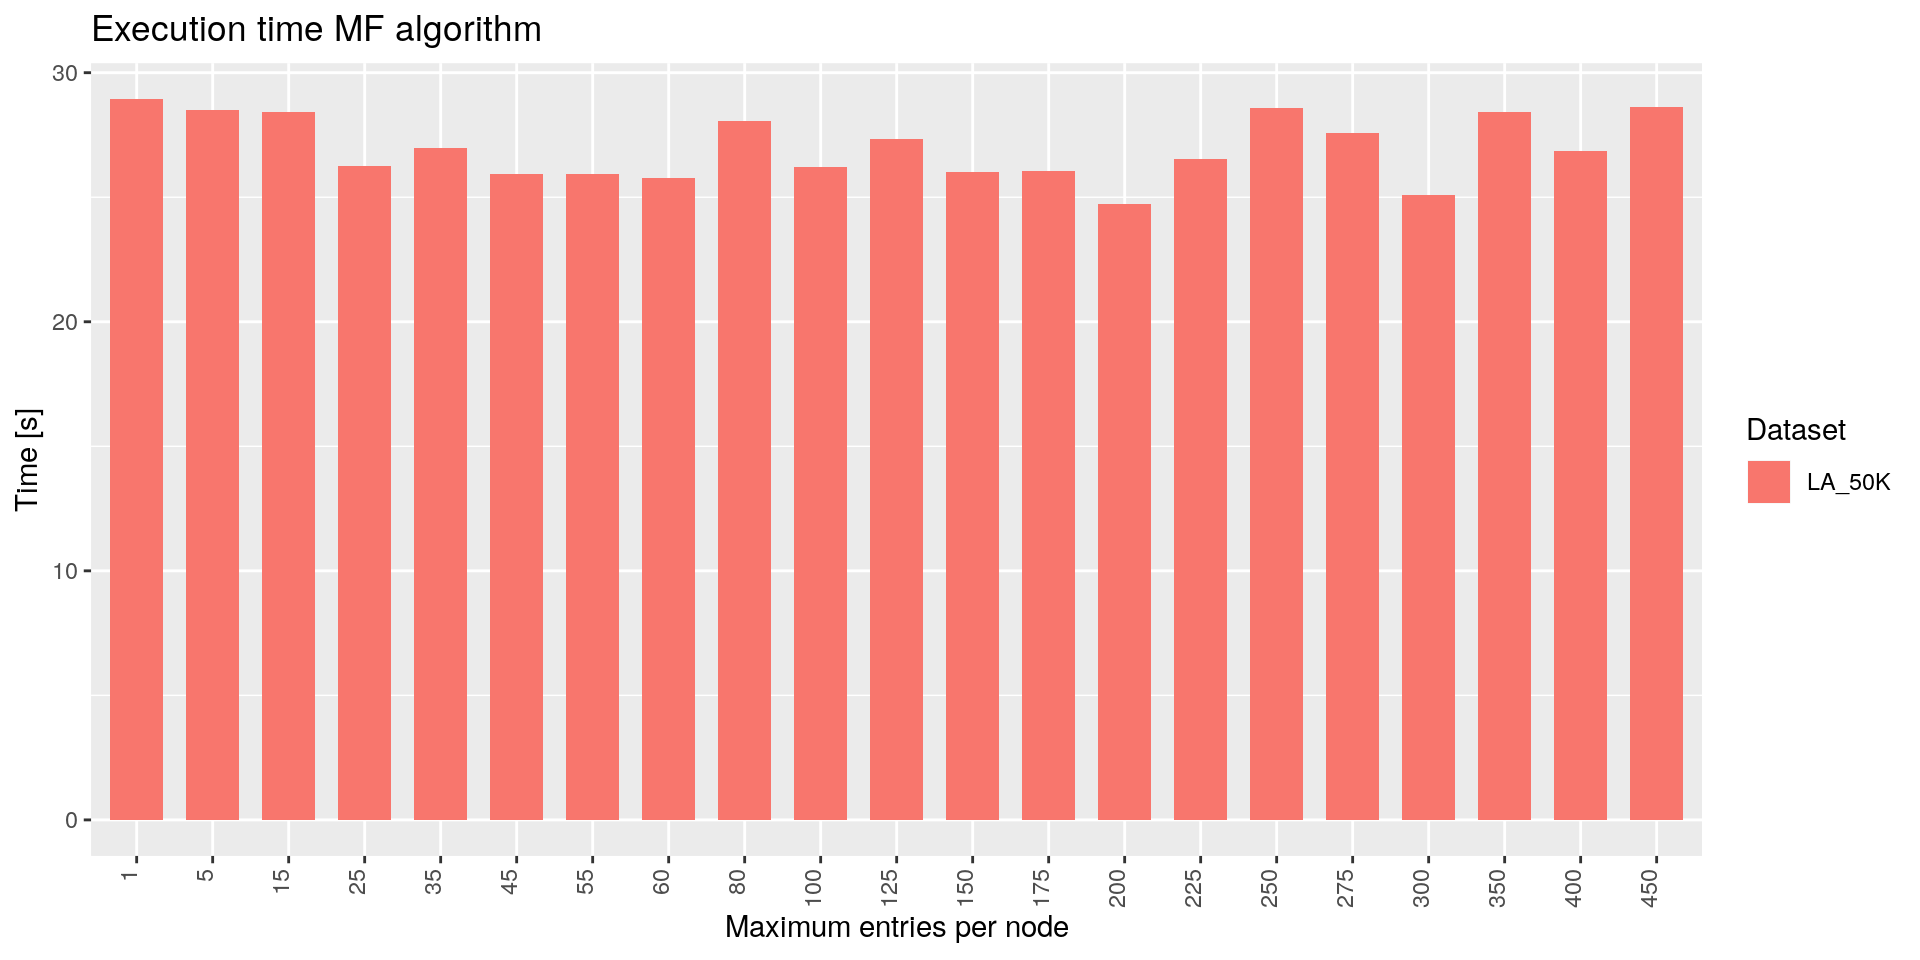
\includegraphics[width=0.66\textwidth]{figures/LA50KMaxEntries.png} \\
    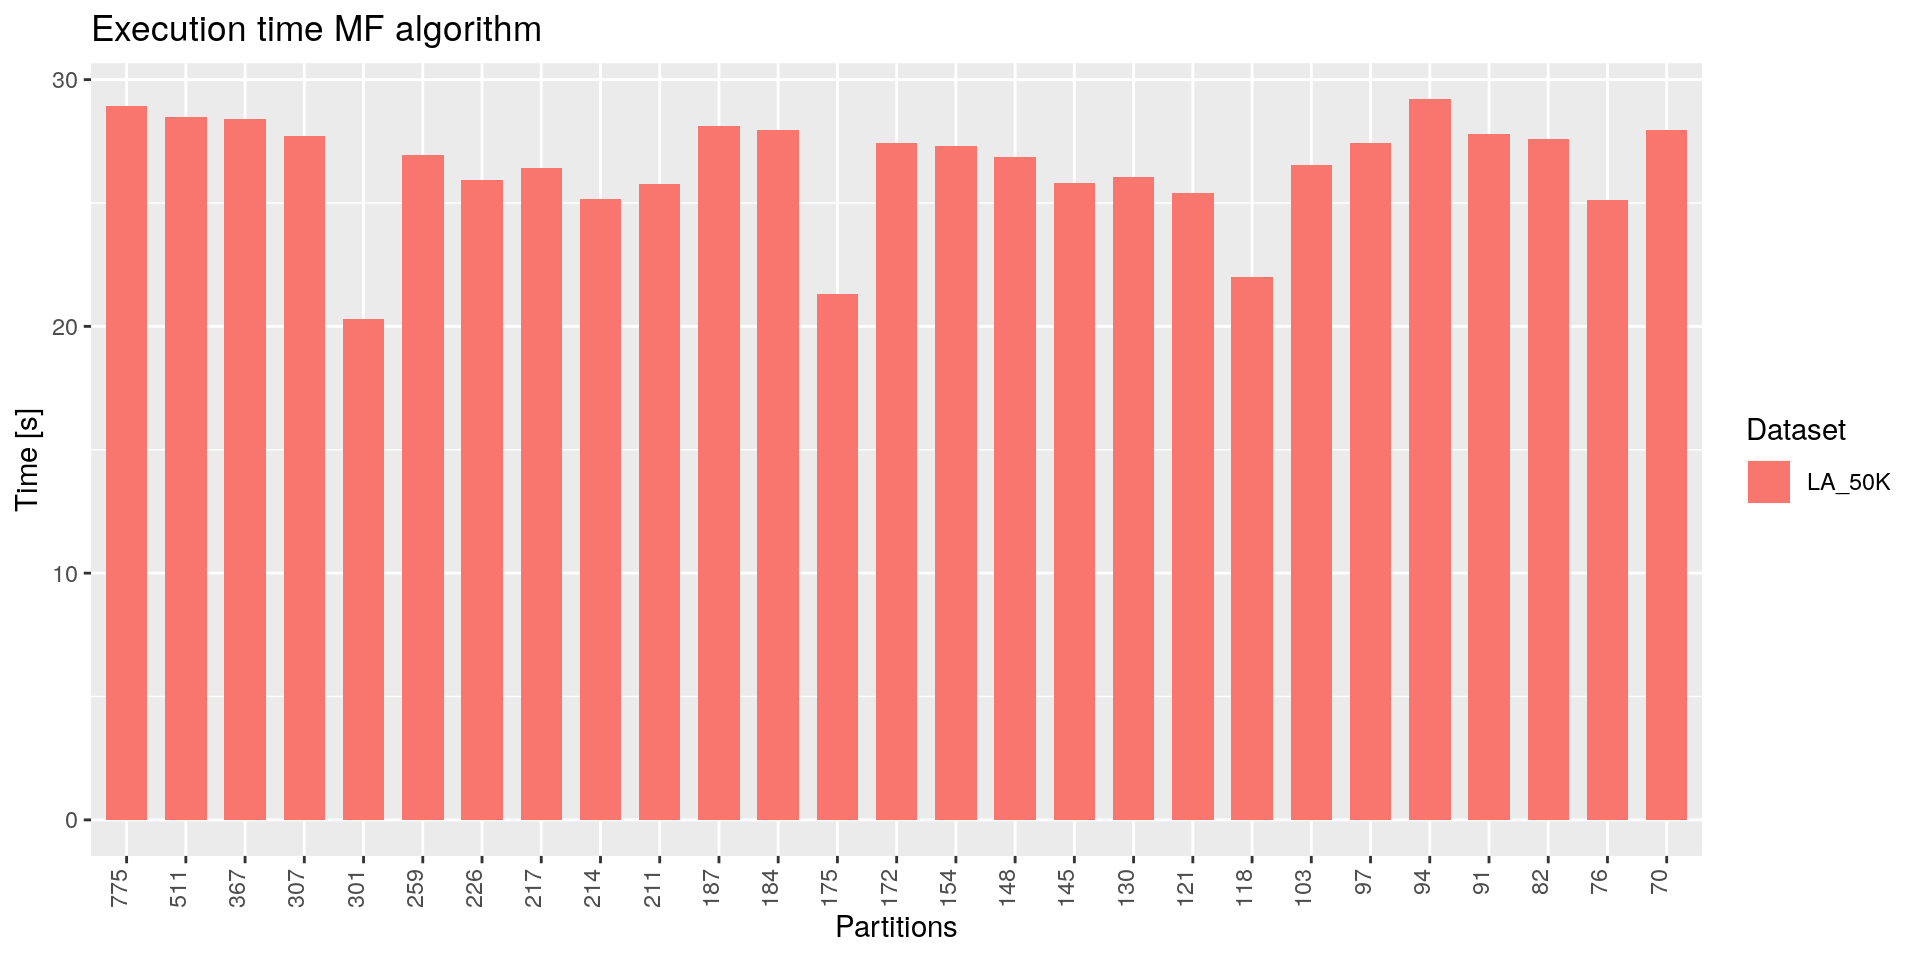
\includegraphics[width=0.66\textwidth]{figures/LA50KPartitions.png}
\end{frame}

\begin{frame}{Extended tests on MF Algorithm (LA\_100K dataset)}
    \centering
    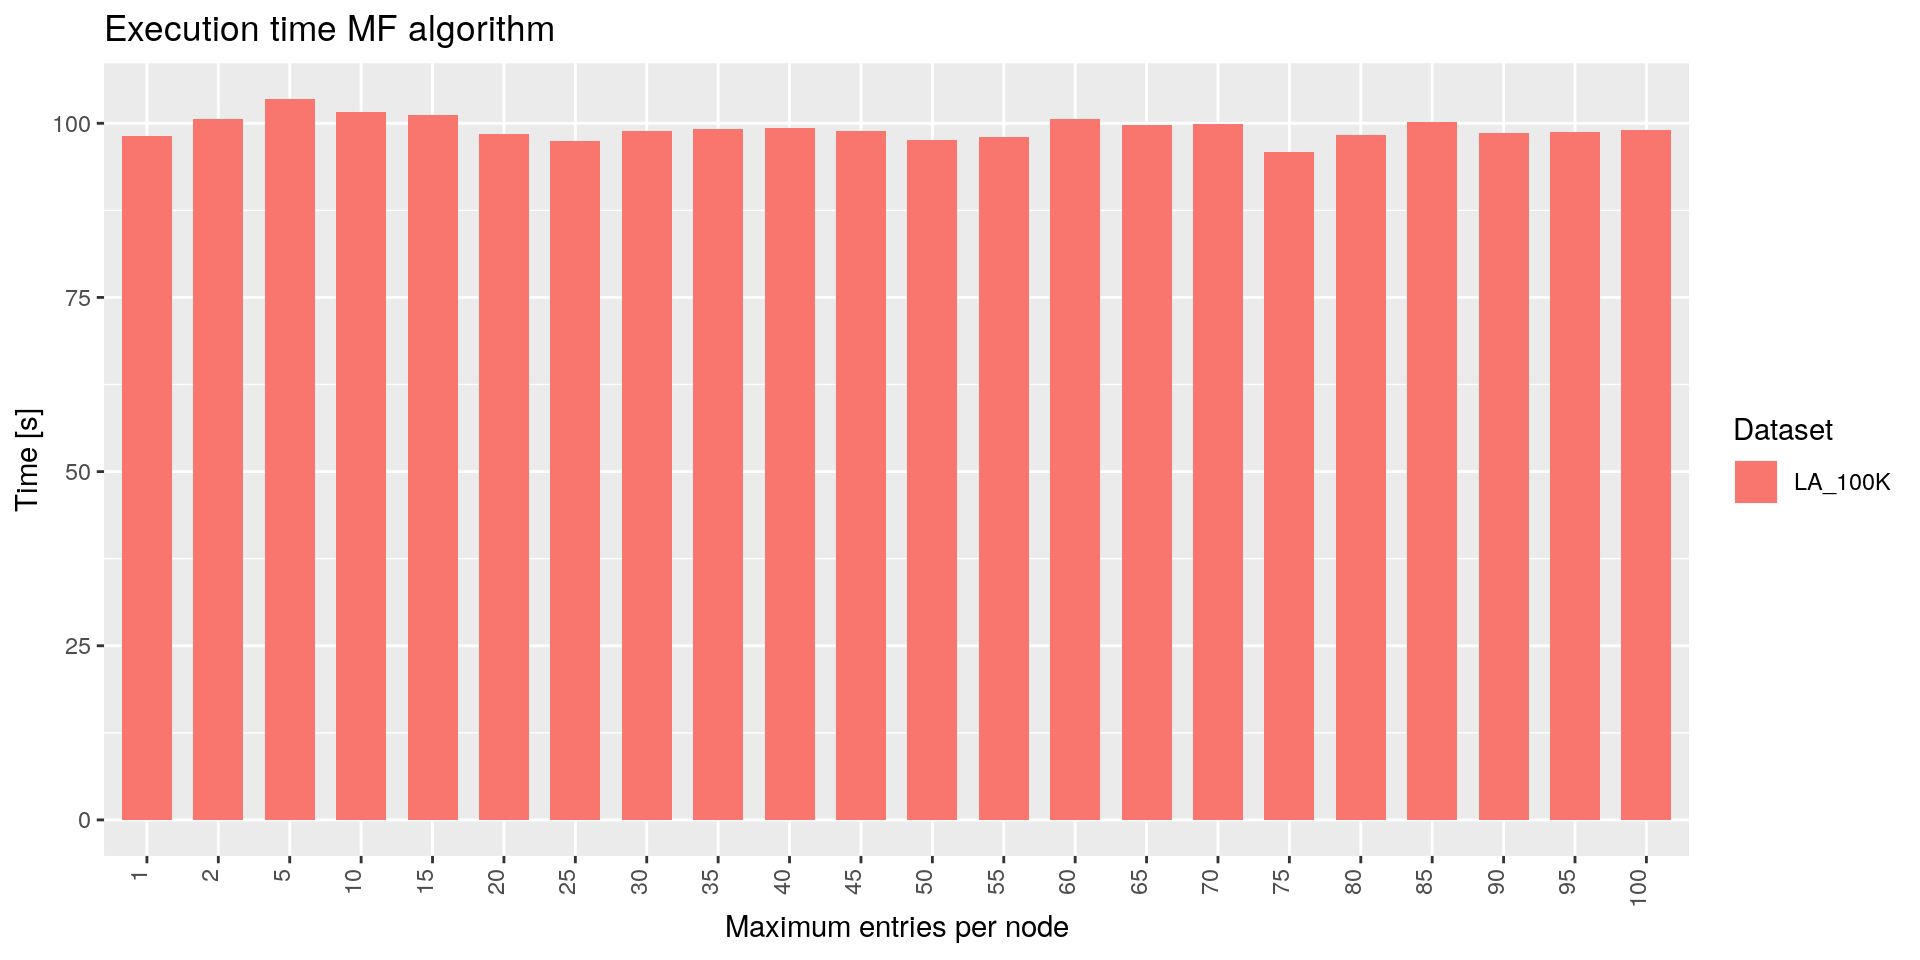
\includegraphics[width=0.66\textwidth]{figures/LA100KMaxEntries.png} \\
    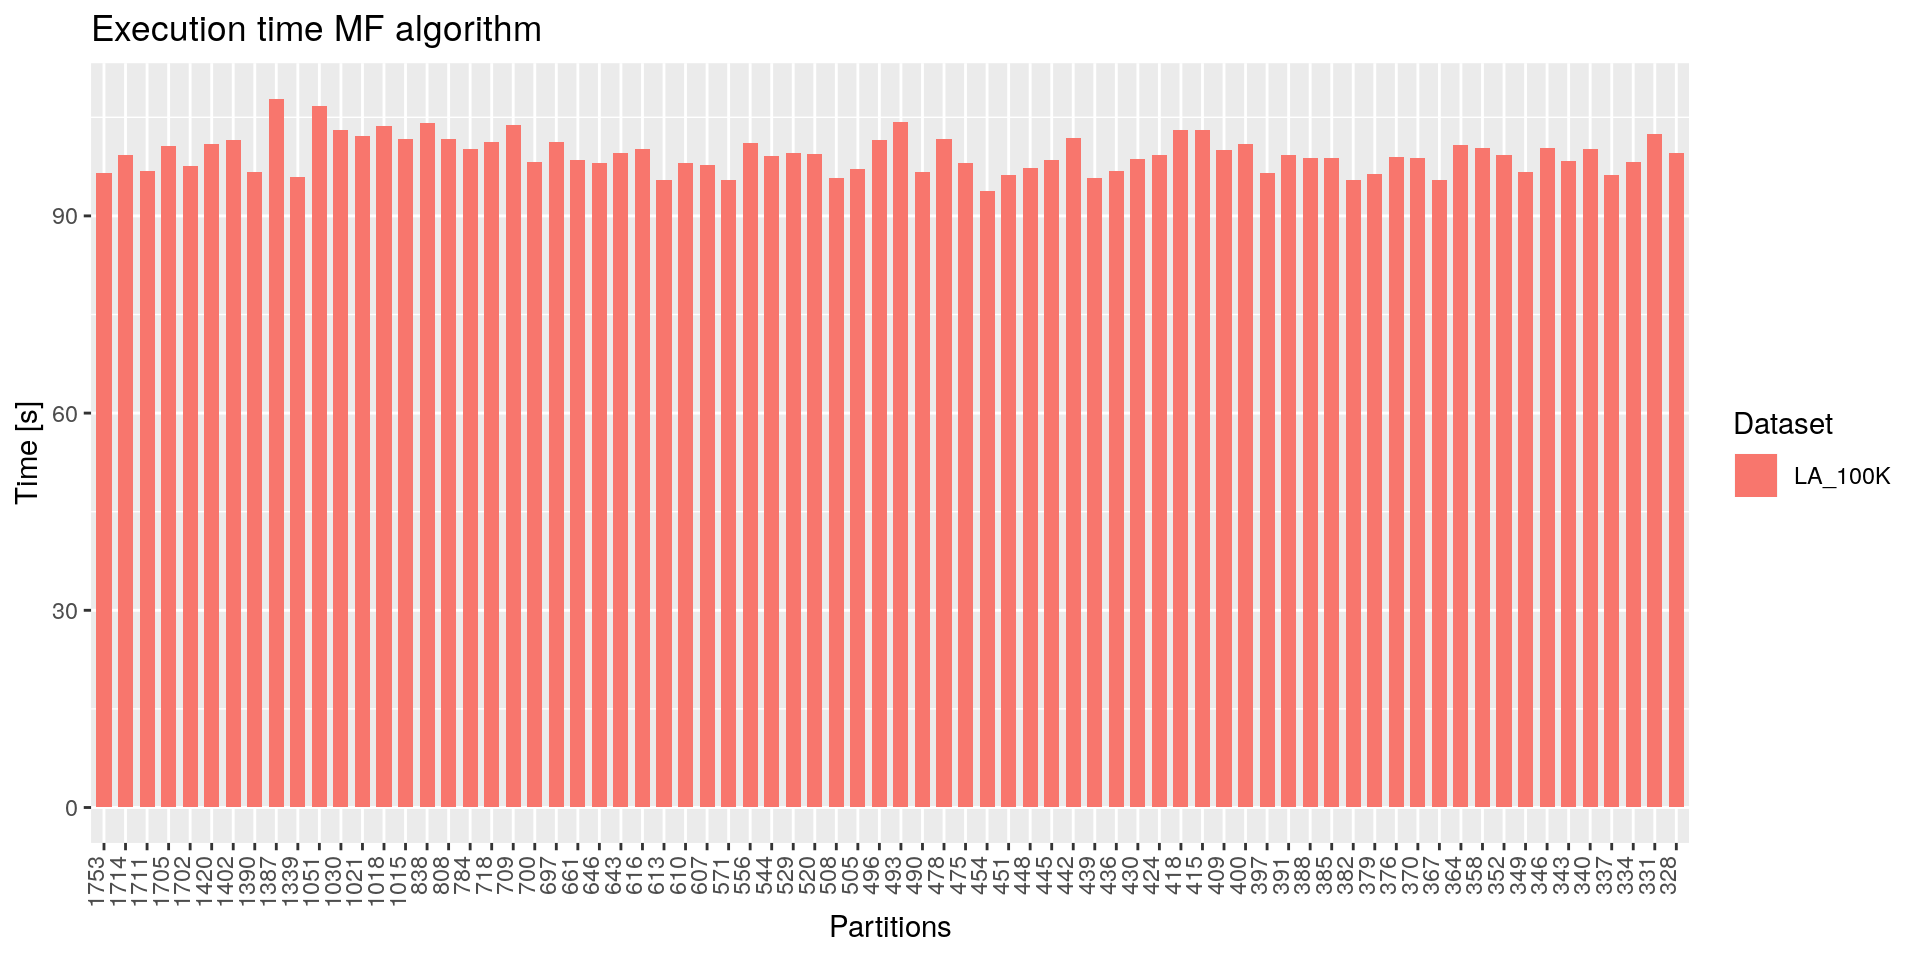
\includegraphics[width=0.66\textwidth]{figures/LA100KPartitions.png}
\end{frame}

\begin{frame}{Extended tests on MF Algorithm (Uniform dataset)}
    \centering
    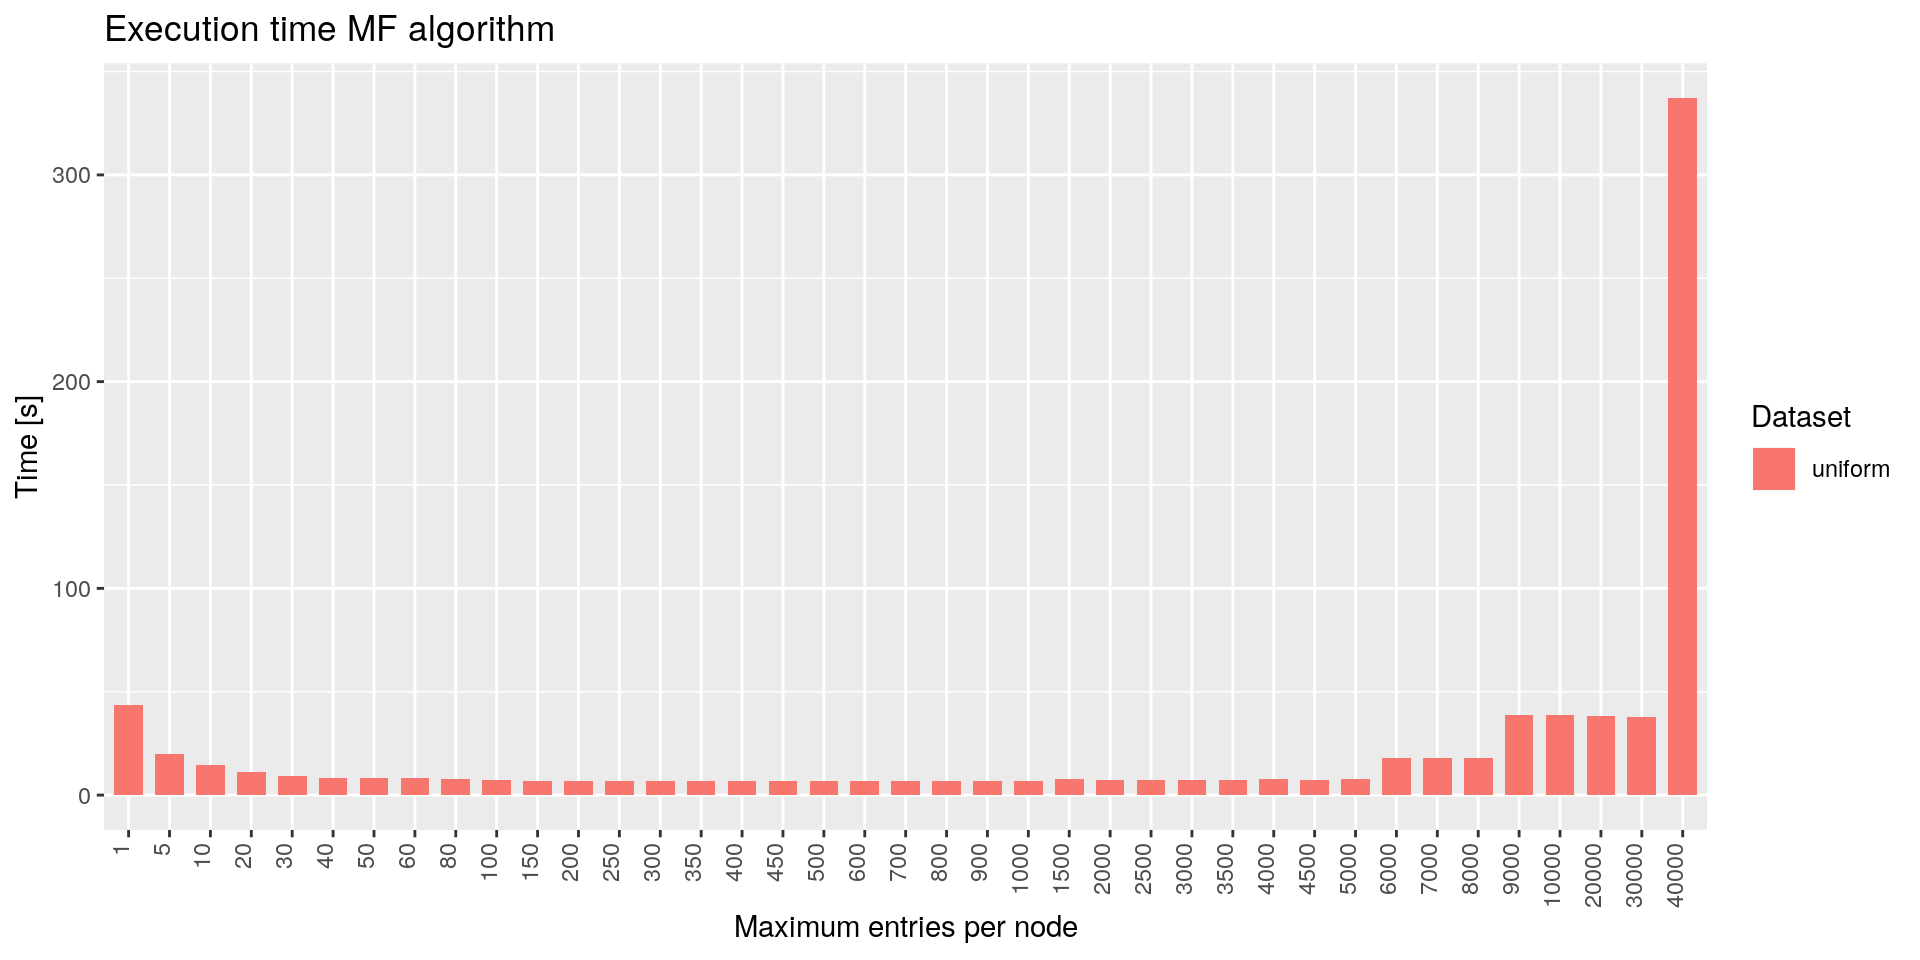
\includegraphics[width=0.66\textwidth]{figures/UniformMaxEntries.png} \\
    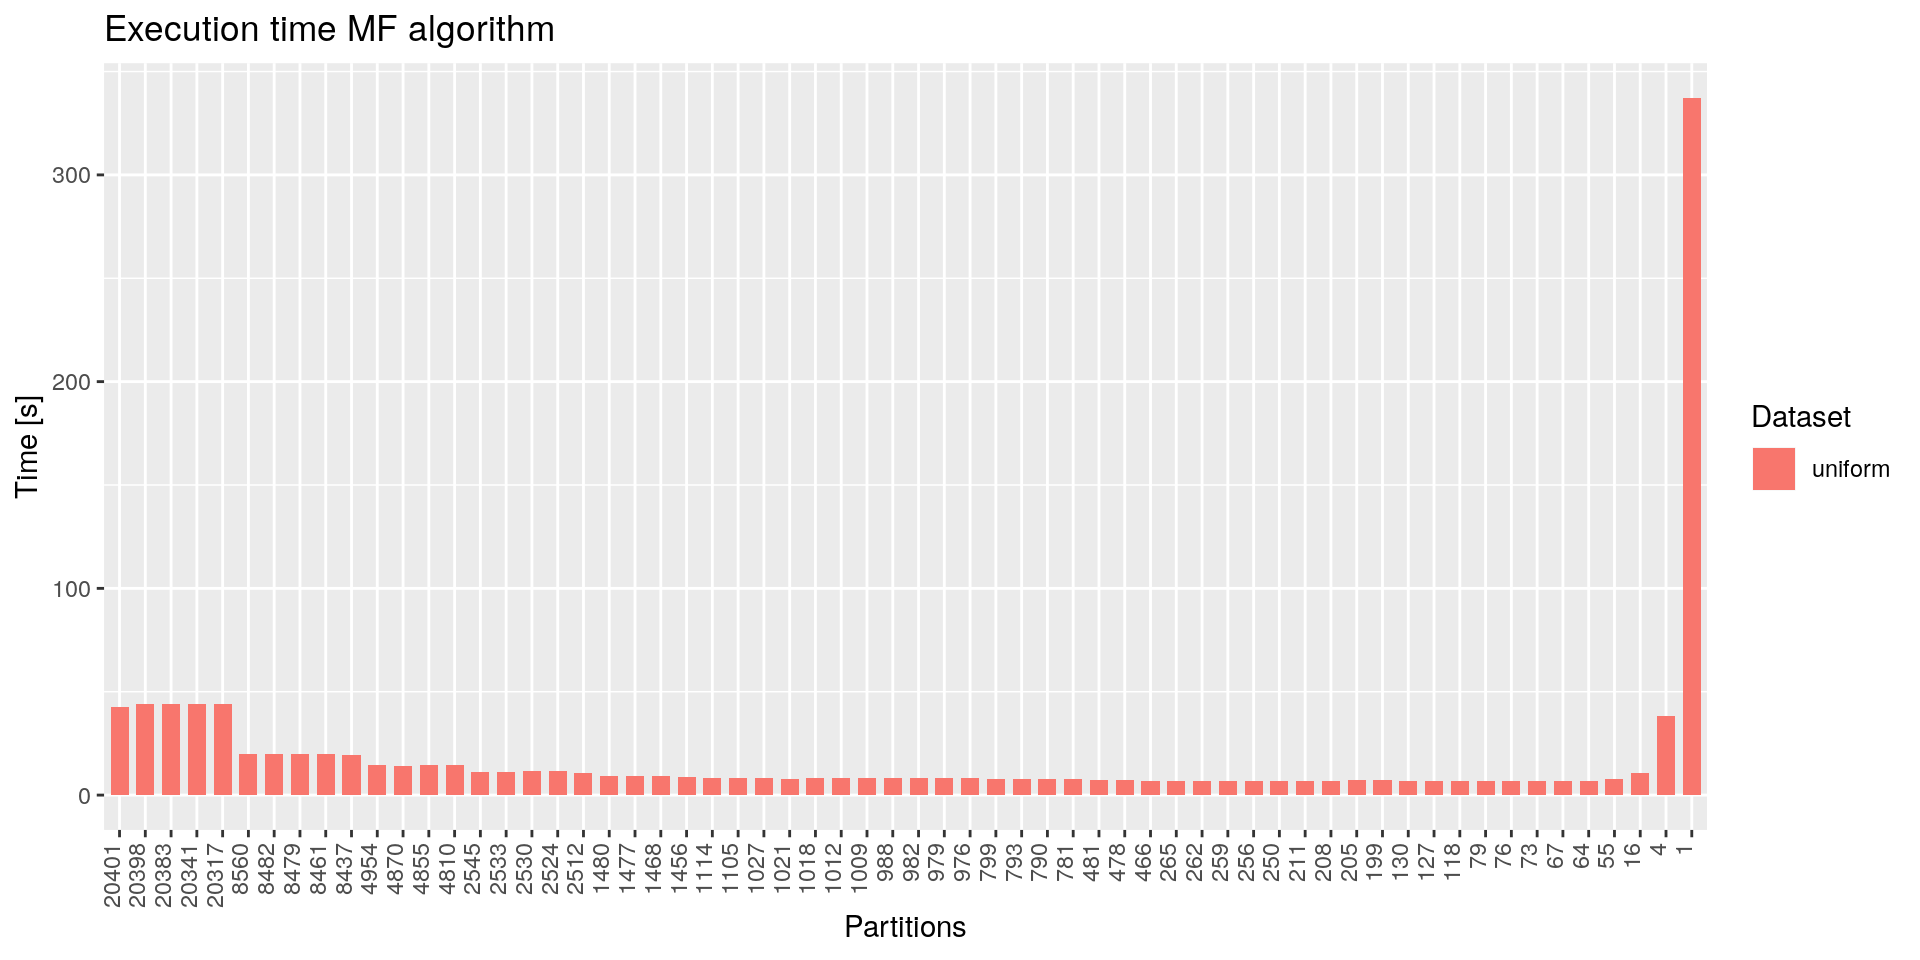
\includegraphics[width=0.66\textwidth]{figures/UniformPartitions.png}
\end{frame}

\section{Debugging FF Algorithm and initial tests}

\begin{frame}{Some remarks (debugging the code)}
    \begin{itemize}
        \item Fixing some issues with the performance in larger datasets.
        \item Join between time intervals works fine with default settings.
        \item We need an additional pruning\footnote{\tiny We can use same LCM strategy than in MF algorithm} after the join of time intervals but data size is much smaller than expected. 
        \item However it still requires to tune its parameters.
        \item It has been difficult to set the parameters for each partitioner.
    \end{itemize}
\end{frame}

\begin{frame}{Some remarks (debugging the code)}
    \centering
    \begin{figure}
        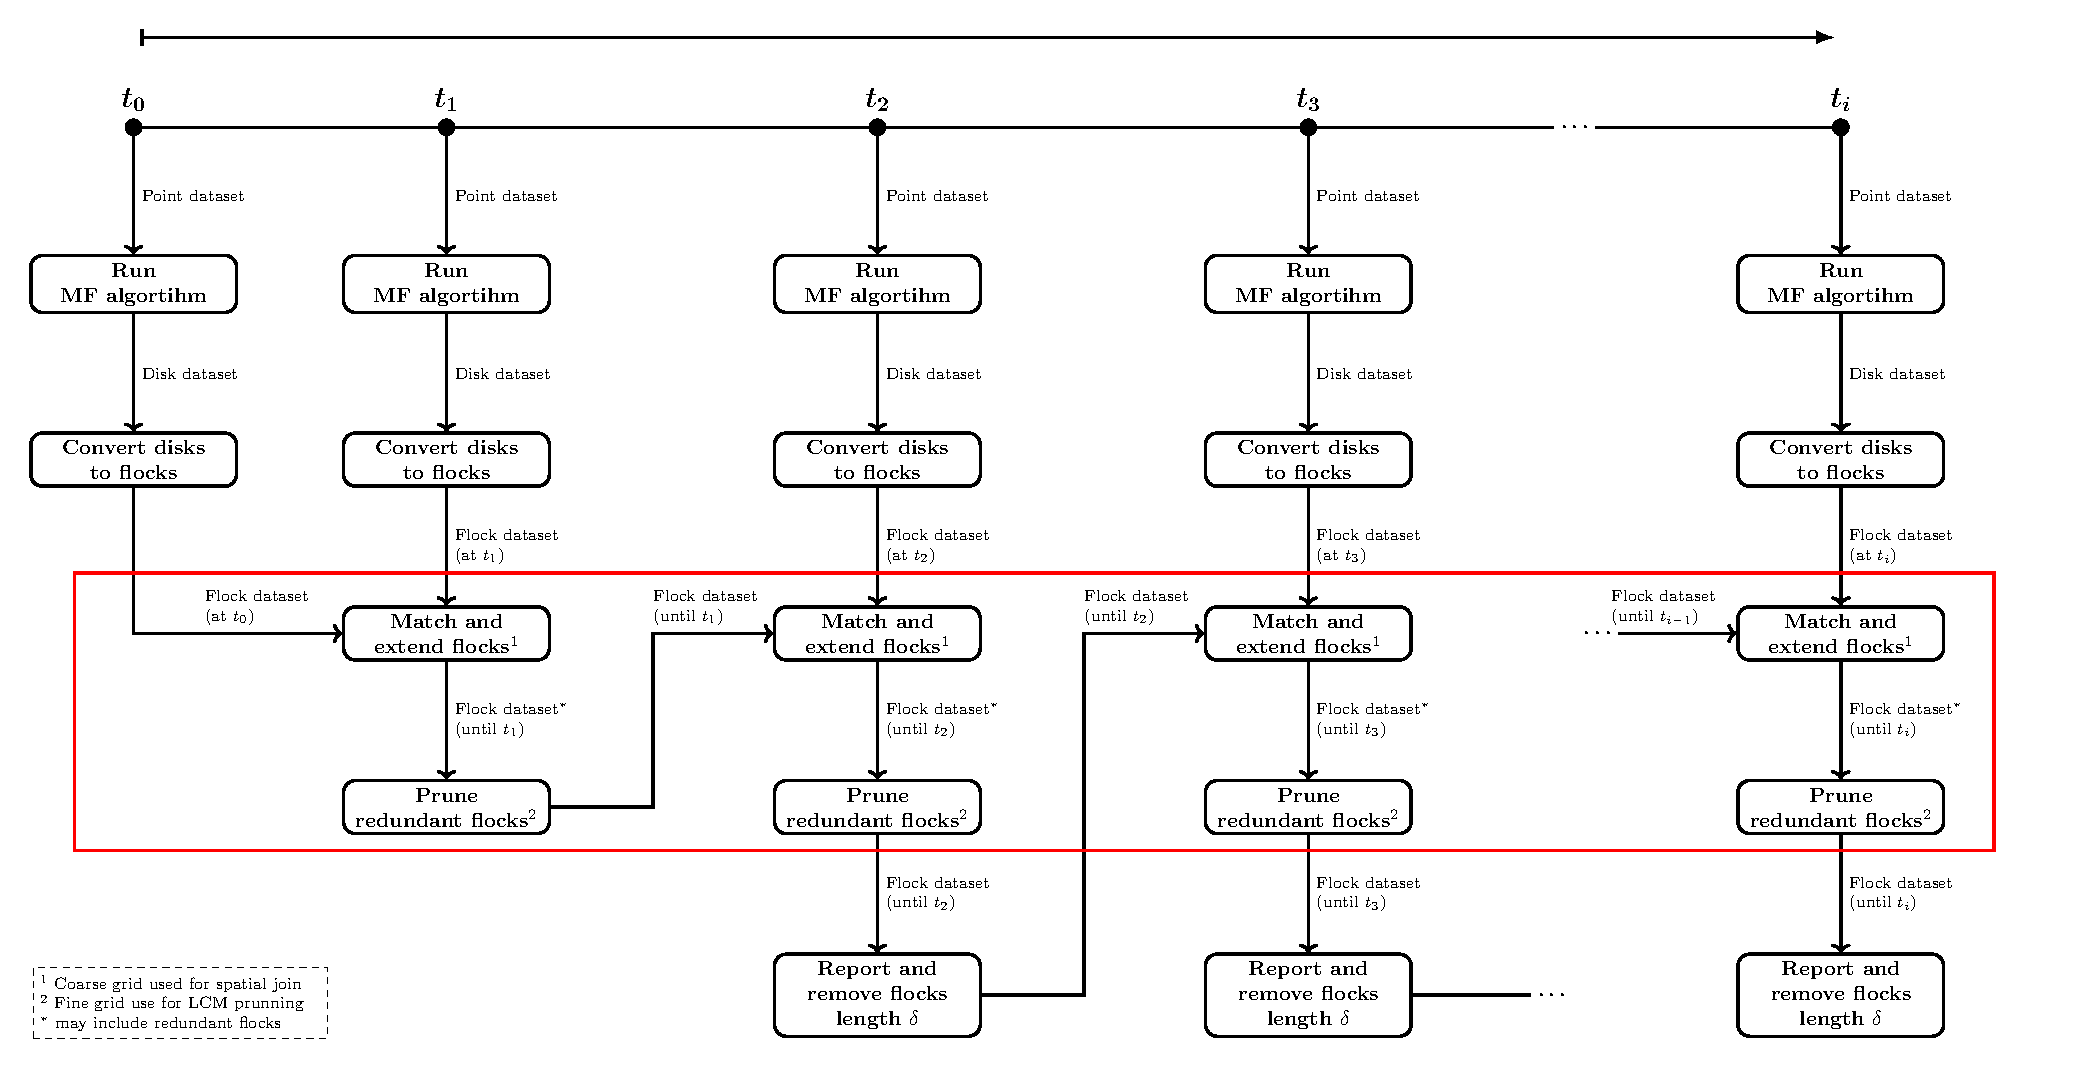
\includegraphics[width=1\textwidth]{figures/FF_flowchart} \\
    \end{figure}
\end{frame}

\begin{frame}{Some remarks (about the partitioners)}
    \begin{itemize}
        \item The size of the sample also plays a role on how to tune the Quadtree and the partitioner.
        \item I have implemented an strategy to infer the size of the sample depending on the size of the dataset.
        \item Overall initial tests run well up to time interval 40 ($\approx$ 60K trajectories per time interval).
    \end{itemize}
\end{frame}

\begin{frame}{Some challenges (about the current scenario)}
    \begin{itemize}
        \item It is clear that in this scenario (number of trajectories increases along time intervals), a fix setting of parameters will not work for all the cases.
        \item I have been working on a strategy to dynamically adjust the parameters but I am still on that.
        \item It should be useful to work with a more stable dataset to test the implementation and then explore the dynamic setting.
    \end{itemize}
\end{frame}

\end{document}
